\documentclass[10pt,colorlinks=true,urlcolor=blue]{moderncv}
\usepackage{todonotes}
\usepackage{ulem}
\usepackage{utopia}
\usepackage[unicode]{hyperref}
\usepackage{color}
\usepackage{pdfpages}
\usepackage{breakurl}
\usepackage[yyyymmdd]{datetime}
\moderncvtheme[blue]{classic}
\usepackage[utf8]{inputenc}
%JLP\usepackage[resetlabels]{multibib}
\usepackage[%
    backend=biber,
    defernumbers=true,
    refsection=section,
    sorting=ydmdt,
    firstinits=false,
    maxbibnames=999]{biblatex}
%\usepackage{etoolbox}
%\addbibresource{peer.bib}
%\addbibresource{pre.bib}
%\addbibresource{talks.bib}
%\addbibresource{other_talks.bib}
%\addbibresource{posters.bib}
\appto{\bibsetup}{\raggedright}
%%
\addbibresource{pubs_peer_reviewed.bib}
\addbibresource{pubs_pre_prints.bib}
\addbibresource{pubs_conf.bib}
\addbibresource{pubs_other.bib}
\addbibresource{pubs_tech_reports.bib}
\addbibresource{pubs_excluded_entries.bib}
\addbibresource{talks_invited.bib}
\addbibresource{talks_other.bib}
\addbibresource{talks_excluded_entries.bib}
\addbibresource[label=posters]{posters.bib}
\newcommand*{\subsubsectionfont}{\uline{\large\mdseries\itshape}}% New subsubsection font
\newcommand*{\subsubsectionstyle}[1]{{\subsubsectionfont\textcolor{color1}{#1}}}
\makeatletter
\NewDocumentCommand{\subsubsection}{sm}{%
  \par\addvspace{1ex}%
  \phantomsection{}% reset the anchor for hyperrefs
  \addcontentsline{toc}{subsubsection}{#2}%
  \begin{tabular}{@{}p{\hintscolumnwidth}@{\hspace{\separatorcolumnwidth}}p{\maincolumnwidth}@{}}%
    \raggedleft\hintstyle{} &{\strut\subsubsectionstyle{#2}}%
  \end{tabular}%
  \par\nobreak\addvspace{0.5ex}\@afterheading}% to avoid a pagebreak after the heading
\makeatother
\DeclareRefcontext{J}{labelprefix=J} %% Peer
\DeclareRefcontext{P}{labelprefix=P} %% Pre-prints
\DeclareRefcontext{I}{labelprefix=I} %% Invited Talks
\DeclareRefcontext{T}{labelprefix=T} %% Other Talks
\DeclareRefcontext{A}{labelprefix=A} %% Abstacts and Posters

% Count total number of entries in each refsection
\AtDataInput{%
  \csnumgdef{entrycount:\therefsection}{%
    \csuse{entrycount:\therefsection}+1}}

% Print the labelnumber as the total number of entries in the
% current refsection, minus the actual labelnumber, plus one
\DeclareFieldFormat{labelnumber}{\mkbibdesc{#1}}    
\newrobustcmd*{\mkbibdesc}[1]{%
  \number\numexpr\csuse{entrycount:\therefsection}+1-#1\relax}

\renewcommand*{\mkbibnamegiven}[1]{%
  \ifitemannotation{highlight}
    {\textbf{#1}}
    {
        \ifitemannotation{trainee}
            {\textit{#1}}
            {#1}
    }
}

\renewcommand*{\mkbibnamefamily}[1]{%
  \ifitemannotation{highlight}
    {\textbf{#1}}
    {
        \ifitemannotation{trainee}
            {\textit{#1}}
            {#1}
    }
}

%\usepackage{pdfpages}
\usepackage{lastpage}
\usepackage{fancyhdr}
\pagestyle{fancy}
\pagenumbering{roman}
\chead{\textbf{Joshua T. Vogelstein, Ph.D.}, Assistant Professor, JHU -- Curriculum Vitae}
\rhead{\textbf{\today}}

\fancyfoot[C]{Page \thepage\ of \pageref*{LastPage}}

\DeclareSortingTemplate{ydmdt}{
  \sort{
    \field{presort}
  }
  \sort[final]{
    \field{sortkey}
  }
  \sort[direction=descending]{
    \field{sortyear}
    \field{year}
  }
  \sort[direction=descending]{
    \field[padside=left,padwidth=2,padchar=0]{month}
    \literal{00}
  }
  \sort[direction=descending]{
    \field[padside=left,padwidth=2,padchar=0]{day}
    \literal{00}
  }
  \sort{
    \field[padside=left,padwidth=4,padchar=0]{volume}
    \literal{0000}
  }
  \sort{
    \field{sorttitle}
  }
}

\usepackage[scale=0.8]{geometry}
\newcommand{\cvdoublecolumn}[2]{%
  \cvline{}{}{%
    \begin{minipage}[t]{\listdoubleitemmaincolumnwidth}#1\end{minipage}%
    \hfill%
    \begin{minipage}[t]{\listdoubleitemmaincolumnwidth}#2\end{minipage}%
    }%
}
%
% usage: \cvreference{name}{address line 1}{address line 2}{address line 3}{address line 4}{e-mail address}{phone number}
% Everything but the name is optxional
% If \addresssymbol, \emailsymbol or \phonesymbol are specified, they will be used.
% (Per default, \addresssymbol isn't specified, the other two are specified.)
% If you don't like the symbols, remove them from the following code, including the tilde ~ (space).

\newcommand{\cvreference}[7]{%
    \textbf{#1}\newline% Name
    \ifthenelse{\equal{#2}{}}{}{\addresssymbol~#2\newline}%
    \ifthenelse{\equal{#3}{}}{}{#3\newline}%
    \ifthenelse{\equal{#4}{}}{}{#4\newline}%
    \ifthenelse{\equal{#5}{}}{}{#5\newline}%
    \ifthenelse{\equal{#6}{}}{}{\texttt{#6}\newline}%
    \ifthenelse{\equal{#7}{}}{}{\phonesymbol~#7}}

  \AtBeginDocument{\recomputelengths}
  \firstname{Joshua T.~}
  \familyname{Vogelstein}
  \address{Assistant Professor, \\
   Department of Biomedical Engineering \\
   Johns Hopkins University \\
   }{}
  \email{jovo@jhu.edu}
  \homepage{jovo.me}


\begin{document}
\pagecolor{white}
\maketitle


\section{Personal Information}

\subsection{Primary Appointment}
\cventry{08/14 -- }{Assistant Professor}{Department of Biomedical Engineering}{JHU}{}{}


\subsection{Joint Appointments}
    \cventry{09/19 -- }{Joint Appointment}{Department of Biostatistics}{Johns Hopkins University (JHU)}{}{}
    \cventry{08/15 -- }{Joint Appointment}{Department of Applied Mathematics and Statistics}{JHU}{}{}
    \cventry{08/14 -- }{Joint Appointment}{Department of Neuroscience}{JHU}{}{}
    \cventry{08/14 -- }{Joint Appointment}{Department of Computer Science}{JHU}{}{}


\subsection{Institutional and Center Appointments}
    \cventry{08/15 -- }{Steering Committee}{Kavli Neuroscience Discovery Institute (KNDI)}{}{}{}
    \cventry{08/14 -- }{Core Faculty} {Institute for Computational Medicine}{JHU}{}{}
    \cventry{08/14 -- }{Core Faculty} {Center for Imaging Science}{JHU}{}{}
    \cventry{08/14 -- }{Assistant Research Faculty}{Human Language Technology Center of Excellence}{JHU}{}{}
    \cventry{10/12 -- }{Affiliated Faculty}{Institute for Data Intensive Engineering and Sciences}{JHU}{}{}


\subsection{Education \& Training}
    \cventry{2003 -- 2009}{Ph.D in Neuroscience}{Johns Hopkins School of Medicine}{\newline Advisor: Eric Young}{\newline \textbf{Thesis:} OOPSI: a family of optical spike inference algorithms for inferring neural connectivity from population calcium imaging }{}{}
    \cventry{2009 -- 2009}{M.S. in Applied Mathematics \& Statistics}{ Johns Hopkins University}{}{}{}
    \cventry{1998 -- 2002}{B.A. in Biomedical Engineering}{Washington University, St.~Louis}{}{}{}


\subsection{Academic Experience}
    \cventry{08/18 -- }{\href{https://www.bme.jhu.edu/graduate/mse/degree-requirements/biomedical-data-science/}{Director of Biomedical Data Science Focus Area}}{Department of Biomedical Engineering, Johns Hopkins University}{}{}{}
    \cventry{05/16 -- }{Visiting Scientist} {Howard Hughes Medical Institute}{Janelia Research Campus}{}{}
    \cventry{10/12 -- 08/14}{Endeavor Scientist}{Child Mind Institute}{}{}{}
    \cventry{08/12 -- 08/14}{Affiliated Faculty}{Kenan Institute for Ethics}{}{}{Duke University}
    \cventry{08/12 -- 08/14}{Adjunct Faculty}{Department of Computer Science, Johns Hopkins University}{}{}{}
    \cventry{12/09 -- 01/11}{Post-Doctoral Fellow}{Department of Applied Mathematics and Statistics}{Supervised by Carey E.~Priebe}{Johns Hopkins University}{\textbf{Research} Statistics of populations of networks.}
    
    \cventry{06/01 -- 09/01}{Research Assistant}{Prof. Randy O'Reilly, Dept.~of Psychology}{}{}{University of Colorado}
    \cventry{06/00 -- 09/00}{Clinical Engineer}{Johns Hopkins Hospital}{}{}{}
    \cventry{06/99 -- 08/99}{Research Assistant under Dr. Jeffrey Williams}{Dept. of Neurosurgery, Johns Hopkins Hospital}{}{}{}
    \cventry{06/98 -- 08/98}{Research Assistant under Professor Kathy Cho}{Dept. of Pathology, Johns Hopkins School of Medicine}{}{}{}


\section{Publications}
%\subsection{Peer Reviewed Articles (accepted, in press, or published)}
%\section{Published Peer-Review Research Articles}

\begin{refsection}[pubs_peer_reviewed.bib] 
%\newrefcontext{J}
\nocite{*}
\defbibnote{a1}{{Note: CV author in bold; Trainees in italics, \\
        \textbf{(55 papers; top 10 cited 3,128 times; H-index 30; 11 first, 10 last, 55 middle authorships)} as of \today}}
\printbibliography[%
    title=\href{https://neurodata.io/publications/\#peer_reviewed}{Published (Peer-Reviewed Research Articles)},%
    prenote=a1,% 
    heading=subbibliography%
    ]
\end{refsection}

%\subsection{Pre-Prints}
\begin{refsection}[pubs_pre_prints.bib] %, pubs_excluded_entries.bib]
%\newrefcontext{P}
\nocite{*}
\printbibliography[%
    title=\href{https://neurodata.io/publications/\#pre_prints}{Submitted (Peer-Review Research Articles)},%
    heading=subbibliography%
    ]
\end{refsection}

\begin{refsection}[pubs_conf.bib]
\nocite{*}
\printbibliography[%
    title=\href{https://neurodata.io/publications/\#conf}{Peer-Reviewed Conference Proceedings},%
    heading=subbibliography%
    ]
\end{refsection}

%\subsection{Pre-Prints}
%\begin{refsection}[pubs_in_prep.bib] %, pubs_excluded_entries.bib]
    %\newrefcontext{P}
%    \nocite{*}
%    \printbibliography[%
%        title=\href{https://neurodata.io/publications/\#pre_prints}{In Preparation (Peer-Review Research Articles)},%
%        heading=subbibliography%
%        ]
%    \end{refsection}

 %\subsection{Pre-Prints}
\begin{refsection}[pubs_tech_reports.bib] %, pubs_excluded_entries.bib]
    %\newrefcontext{P}
\nocite{*}
\printbibliography[%
    title=\href{https://neurodata.io/publications/\#pre_prints}{Technical Reports},%
    heading=subbibliography%
    ]
\end{refsection}

%\subsection{Pre-Prints}
\begin{refsection}[pubs_other.bib] %, pubs_excluded_entries.bib]
%\newrefcontext{P}
\nocite{*}
\printbibliography[%
    title=\href{https://neurodata.io/publications/\#other}{Other Publications},%
    heading=subbibliography%
    ]
\end{refsection}
    
    
    
%\nopagecolor
%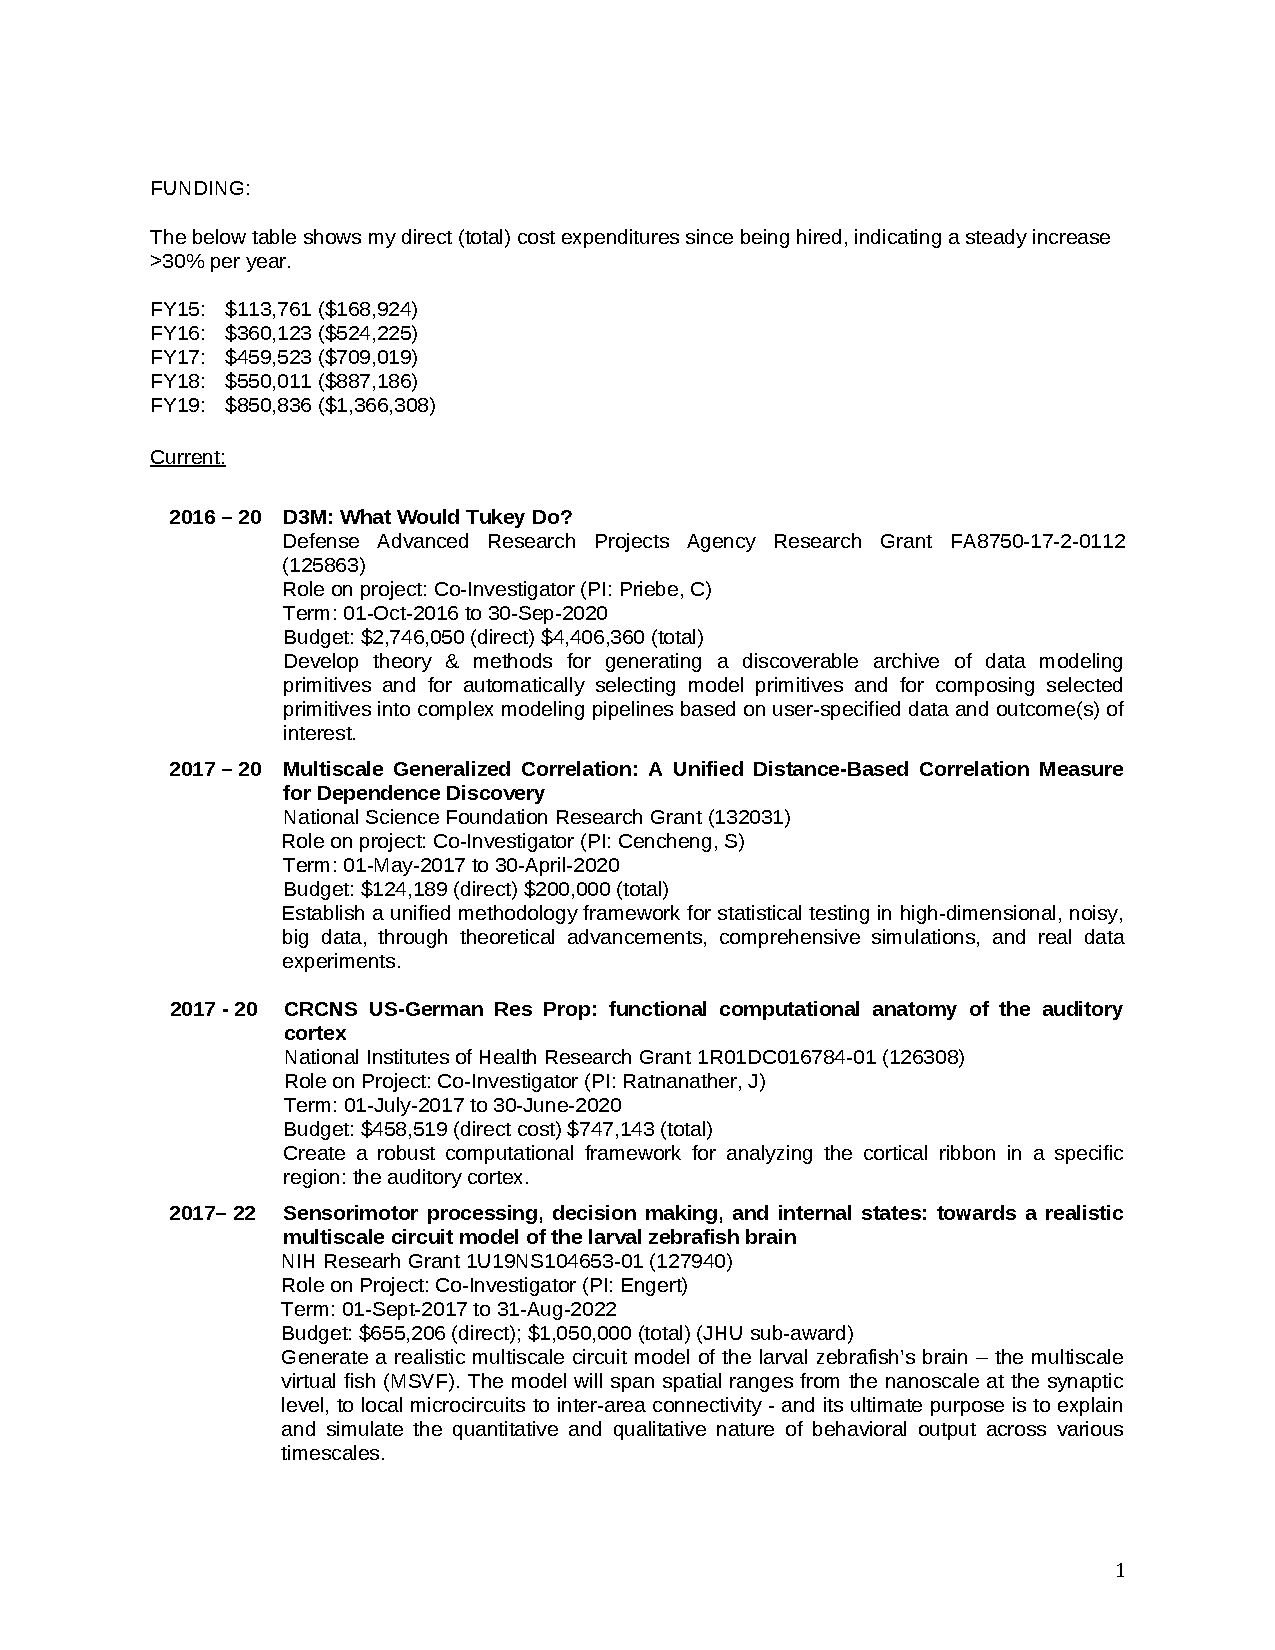
\includepdf[pages=-]{funding_history_2019_01_03.pdf}
% \newpage
\section{Funding}

The below table shows my direct (total) cost expenditures since being hired, indicating a steady increase >30\% per year.

\centering
\begin{tabular}{p{3cm}p{2cm}p{3cm}}
Financial Year & Direct & Total \\
2015: & \$113,761 & \$168,924 \\
2016: & \$360,123 & \$524,225 \\
2017: & \$459,523 & \$709,019 \\
2018: & \$550,011 & \$887,186 \\
2019: & \$850,836 & \$1,366,308
\end{tabular}


\subsection{Current}

\cventry{2020 – 2025}{CAREER: Foundational Statistical Theory and Methods for Analysis of Populations of Attributed}{}
{\newline NSF 17-537
\newline Role on project: Principal Investigator
\newline Term: {01-Mar-2020} to 31-Dec-2025
\newline Budget: \$384,873 (direct) \$245,357 (indirect) \$630,230 (total)
\newline The goal is to establish foundational theory and methods for analyzing populations of
attributed connectomes}{}{}{}{}

\cventry{2019 -- 2022}{Accessible technologies for high-throughput, whole-brain reconstructions of molecularly characterized mammalian neurons}{}
{\newline NIH RO1 Research Grant
\newline Role on project: Co-Investigator (PI: Muller, Miller)
\newline Term: 01-Sept-2019 to 31-Aug-2022
\newline Total budget: \$753,974 (direct) \$426,471 (indirect) \$1,180,445 (total cost)
\newline The overall goal of the proposal is to develop technologies for the brain wide reconstruction
of axonal arbors of molecularly defined neurons. The proposal aims at overcoming barriers
in neuronal labeling, imaging and computation to achieve this goal, and to develop a
technology platform that can be scaled to all neurons of the brain}{}{}{}{}

\cventry{2019 – 2020}{Reproducible imaging-based brain growth charts for psychiatry}{}
{\newline NIH R01 Research Grant 
\newline Role on project: Co-Investigator (PI: Saterthwaite)
\newline Term: 01-Aug-2019 to 31-May-2020
\newline Budget: \$231,276 (direct) \$131,585 (indirect) \$362,861 (total cost)
\newline Aggregate, harmonize, and analyze existing large-scale pediatric neuroimaging datasets to
identify normative and clinical brain growth curves}{}{}{}{}

\cventry{2019 -- }{Microsoft Research Award}{}
{\newline Mircosoft Research Gift
\newline Role on Project: Principal Investigator
\newline Term: Unrestricted Gift
\newline Budget: \$50,000 (total cost)
\newline Research and development of neuroscience and connectomes around neuronal circuit and
system modeling, application of time-series-of-graphs and dynamics to neuronal signaling
analysis and connectomes, and in the abstractions of matter, math, machines that point
toward complex systems composed of low-level components}{}{}{}{}

\cventry{2018 – 2020}{Lifelong Learning Forests}{}
{\newline Defense Advanced Research Projects Agency Research Grant FA8650-18-2-7834
(128567)
\newline Role on Project: Principal Investigator
\newline Term: 01-Jul-2018 to 30-Jun-2020
\newline Budget: \$1,123,474 (direct) \$715,834 (indirect) \$1,839,308 (total cost)
\newline Lifelong Learning Forests (L2Fs) will learn continuously, selectively adapting to new
environments and circumstances utilizing top-down feedback to impact low-level
processing, with provable statistical guarantees, while maintaining computational tractability
at scale}{}{}{}{}

\cventry{2018 – 2021}{SemiSynBio: Collaborative Research: YeastOns: Neural Networks Implemented in Communication Yeast Cells}{}
{\newline National Science Foundation Research Grant (129439)
\newline Role on project: Co-Investigator (PI: Schuman)
\newline Term: 01-Jul-2018 to 30-Jun-2021
\newline Budget: \$172,971 (direct) \$90,971 (indirect) \$263,942 (total cost)
\newline Provide neuroscience and machine learning expertise to guide the design of the
computational learning capabilities of the system}{}{}{}{}

\cventry{2018 – 2019}{Connectome Coding at the Synaptic Scale}{}
{\newline Schmidt Science Foundation (128503)
\newline Role on Project: Principal Investigator
\newline Term: 01-Jan-2018 to 31-Dec-2019
\newline Budget: \$250,000 (total cost)
\newline Study learning and plasticity at an unprecedented scale, revealing the dynamics of large
populations of synapses comprising an entire local cortical circuit. No previously conducted
experiment could answer the questions about the dynamics of large populations of
synapses, which is crucial to understanding the learning process}{}{}{}{}

\cventry{2017 – 2021}{Continual Learning Across Synapses, Circuits, and Brain Areas}{}
{\newline Defense Advanced Research Projects Agency Research Grant FA8650-18-2-7834 (129061)
\newline Role on project: Co-Investigator (PI: Tolias)
\newline Term: 01-Nov-2017 to 30-Oct-2021
\newline Budget: \$486,666 (direct) \$310,049 (indirect) \$796,715 (total cost)
\newline Develop the pre-processing analysis pipeline for the imaging data collected in this project}{}{}{}{}

\cventry{2017 – 2020}{NeuroNex Innovation Award: Towards Automatic Analysis of Multi-Terabyte Cleared Brains}{}
{\newline National Science Foundation 1707298
\newline Role on Project: Principal Investigator
\newline Term: 01-Sept-2017 to 31-Aug-2020 (No Cost Extension)
\newline Budget: \$588,758 (direct) \$371,241 (indirect) \$959,999 (total cost)
\newline We propose to lower the barrier to connecting data to analyses and models by providing a
coherent cloud computational ecosystem that minimizes current bottlenecks in the scientific
process}{}{}{}{}

\cventry{2017 – 2022}{Sensorimotor processing, decision making, and internal states: towards a realistic multiscale circuit model of the larval zebrafish brain}{}
{\newline NIH Research Grant 1U19NS104653-01 (127940)
\newline Role on Project: Co-Investigator (PI: Engert)
\newline Term: 01-Sept-2017 to 31-Aug-2022
\newline Budget: \$655,206 (direct) \$394,794 (indirect) \$1,050,000 (total cost) (JHU sub-award)
\newline Generate a realistic multiscale circuit model of the larval zebrafish’s brain – the multiscale
virtual fish (MSVF). The model will span spatial ranges from the nanoscale at the synaptic
level, to local microcircuits to inter-area connectivity - and its ultimate purpose is to explain
and simulate the quantitative and qualitative nature of behavioral output across various
timescales}{}{}{}{}

\cventry{2017 – 2020}{CRCNS US-German Res Prop: functional computational anatomy of the auditory cortex}{}
{\newline National Institutes of Health Research Grant 1R01DC016784-01 (126308)
\newline Role on Project: Co-Investigator (PI: Ratnanather, J)
\newline Term: 01-July-2017 to 30-June-2020
\newline Budget: \$458,519 (direct) \$288,624 (indirect) \$747,143 (total cost)
\newline Create a robust computational framework for analyzing the cortical ribbon in a specific
region: the auditory cortex}{}{}{}{}

\cventry{2017 – 2020}{Multiscale Generalized Correlation: A Unified Distance-Based Correlation Measure for Dependence Discovery}{}
{\newline National Science Foundation Research Grant (132031)
\newline Role on project: Co-Investigator (PI: Cencheng, S)
\newline Term: 01-May-2017 to 30-April-2020
\newline Budget: \$124,189 (direct) \$75,811 (indirect) \$200,000 (total cost)
\newline Establish a unified methodology framework for statistical testing in high-dimensional, noisy,
big data, through theoretical advancements, comprehensive simulations, and real data
experiments}{}{}{}{}

\cventry{2016 – 2020}{D3M: What Would Tukey Do?}{}
{\newline Defense Advanced Research Projects Agency Research Grant FA8750-17-2-0112 (125863)
\newline Role on project: Co-Investigator (PI: Priebe, C)
\newline Term: 01-Oct-2016 to 30-Sep-2020
\newline Budget: \$2,746,050 (direct) \$1,660,310 (indirect) \$4,406,360 (total cost)
\newline Develop theory and methods for generating a discoverable archive of data modeling
primitives and for automatically selecting model primitives and for composing selected primitives into complex
modeling pipelines based on user-specified data and outcome(s) of interest}{}{}{}{}


%%%%%%%%%%%%%%%%%%%%%%%%%%%%%%%%%%%%%%%%%%%%%%%%%%%%%%%%%%%
\subsection{Pending}

\cventry{2020 – 2023}{Graspy: A python package for rigorous statistical analysis of populations of attributed connectomes}{}
{\newline NIH MN-19-147
\newline Role on project: Principal Investigator
\newline Term: {01-Mar-2020} to 30-June-2023
\newline Budget: \$861,240 (direct) \$549,039 (indirect) \$1,410,279 (total)
\newline The goal of this project is to establish a state-of-the-art toolbox for analysis of
connectomes, spanning taxa, scale, and complexity. More specifically, we will develop and
extend implementations to enable neurobiologists to 1) estimate latent structure from
attributed connectomes, (2) identify meaningful clusters among populations of
connectomes, and (3) detect relationships between connectomes and multivariate
phenotypes, such as behavior, genetics, and physiology}{}{}{}{}

\cventry{2020 – 2022}{High throughput mapping pipeline for incomplete and censored neuroimaging data}{}
{\newline NIH / MH-19-148
\newline Role on Project: Co-Investigator (PI: Miller)
\newline Term: 01-Mar-2020 to 30-Nov-2022
\newline Budget: \$1,107,698 (direct) \$637,159 (indirect) \$1,744,857 (total)
\newline Develop technologies to map brain coordinates on incomplete MRI brain imaging data}{}{}{}{}


\cventry{2020 – 2025}{NeuroNex: Enabling Identification and Impact of Synaptic Weight in Functional Networks}{}
{\newline NSF 19-563
\newline Role on project: Co-Investigator (PI: Harris)
\newline Term: 01-April 2020 to 31-March-2025
\newline Budget: \$609,294 (direct) \$388,425 (indirect) \$997,719 (total)
\newline Develop the requisite technology to understand the impact of synaptic weight on functional
networks}{}{}{}{}

\cventry{2020 – 2025}{Identifying Neurobehavioral Pathways for Cannabis Use Disorder: Multimodal MRI Investigations of Control and Reward Neural Networks}{}
{\newline NIH18-062 - National Institute on Drug Abuse
\newline Role on project: Co-Investigator (PI: Hanson)
\newline Term: 01-April-2020 to 31-March-2025
\newline Budget: \$234,338 (direct) \$149,389 (indirect) \$383,727 (total)
\newline This project will connect strong behavioral markers of addiction risk, measures of drug use,
and measures of brain network connectivity to aid in understanding what causes drug use,
versus what is a consequence of it}{}{}{}{}

\cventry{2020 – 2023}{A Novel Framework for Mapping Brain Dynamics and Substrates of Human Cognition Across Species}{}
{\newline NIH MH-20-120
\newline Role on project: Co-Investigator (PI: Milham)
\newline Term: 01-July-2020 to 30-June-2023
\newline Budget: \$178,898 (direct) \$114,047 (indirect) \$292,945 (total)
\newline Develop and apply modern alignment methods to compare and contrast human and non-
human brain imaging}{}{}{}{}

\cventry{2020 – 2023}{MBAc: Mouse Brain Atlasing in the Cloud}{}
{\newline NIH MN-19-147
\newline Role on project: Co-Investigator (PI: Osten)
\newline Term: 01-July-2020 to 30-June-2023
\newline Budget: \$1,520,570 (direct) \$969,363 (indirect) \$2,489,933 (total)
\newline Develop and disseminate CloudReg, a cloud brain atlasing tool for microscale whole
mouse brains}{}{}{}{}

\cventry{2020 – 2024}{Exploiting latent structure for efficient and robust inference}{}
{\newline NSF
\newline Role on project: Co-Investigatror (PI: Priebe)
\newline Term: 01-July-2020 to 30-June-2024
\newline Budget: \$999,330 (direct) \$505,332 (indirect) \$1,504,662 (total)
\newline Develop theory and methods for analysis of networks and populations thereof}{}{}{}{}

\cventry{2020 – 2024}{Distributed ensemble neural representations of anxiety states}{}
{\newline NIH 0 NS 18-303 BrainInitiative RO1
\newline Role on project: Co-Investigator (PI: Adwanikar)
\newline Term: 01-July-2020 to 30-June-2024
\newline Budget: \$2,672,969 (total)
\newline Imaging the coordinated, multi-area, ensemble neural signaling of anxiety and attention
states at cellular-resolution in freely behaving mice}{}{}{}{}

\cventry{2020 – 2025}{The NKI-Rockland Sample II: An open resource of multimodal brain, physiology, and behavior data from a community lifespan sample}{}
{\newline NIH 19-056
\newline Role on project: Co-Investigator (PI: Milham)
\newline Term: 01-July-2020 to 30-June-2025
\newline Budget: \$30,713 (direct) \$48,178 (indirect) \$78,891 (total)
\newline We will continue collecting, organizing, and analyzing another cohort of the NKI-Rockland
Sample}{}{}{}{}





%%%%%%%%%%%%%%%%%%%%%%%%%%%%%%%%%%%%%%%%%%%%%%%%%%%%%%%%%%%

\subsection{Previous}
\cventry{2017 – 2018}{The Brain Ark}{}
{\newline Defense Advance Research Project Agency Grant 90076467
\newline Role of the Project: Principal Investigator
\newline Budget: \$56,499.08 (direct) \$35,876.92 (indirect) \$92,376 (total cost)
\newline Characterize the statistical properties of the individual graphs, to identify circuit motifs,
both that specialize in a species specific fashion, and that are preserved across species.
As a test, will compare the connectomes of sea lions and coyotes}{}{}{}{}

\cventry{2017 – 2018}{The International Brain Station}{}
{\newline The Kavli Foundation 90071826
\newline Role of the Project: Principal Investigator
\newline Budget: \$50,000 (direct) \$50,000 (total cost)
\newline Take the first few steps towards building the international brain station}{}{}{}{}

\cventry{2017 – 2018}{Brain Comp Infra: EAGER: BrainLab CI: Collaborative, Community Experiments}{}
{\newline National Science Foundation ACI-1649880
\newline Role of Project: Co-Investigator (PI: Miller, Burns)
\newline Budget: \$180,736 (direct) \$113,863 (indirect) \$294,599 (total cost)
\newline The BrainLab CI prototype system will deploy an experimental-management
infrastructure that allows users to construct community-wide experiments that implement
data and metadata controls on the inclusion and exclusion of data}{}{}{}{}

\cventry{2016 – 2019}{A Scientific Planning Workshop for Coordinating Brain Research Around the Globe
National Science Foundation 1637376 Part 1 of 2}{}
{\newline Role of the Project: Principal Investigator
\newline Budget: \$97,950 (direct) \$97,950 (total cost)
\newline This travel grant is for the expressed purposes of gathering researchers from around the
globe to discuss the new way to further brain research during part one of a two day
conference}{}{}{}{}

\cventry{2016 – 2019}{A Scientific Planning Workshop for Coordinating Brain Research Around the Globe
National Science Foundation 1637376 Part 2 of 2}{}
{\newline Role of the Project: Principal Investigator
\newline Budget: \$14,491 (direct) \$1,836 (indirect) \$16,327 (total cost)
\newline This travel grant is for the expressed purposes of gathering researchers from
around the globe to further discuss advancements in brain research during the
second part of a two day conference}{}{}{}{}

\cventry{2015 – 2018}{From RAGs to Riches: Utilizing Richly Attributed Graphs to Reason from}{}
{\newline Defense Advance Research Project Agency Grant N66001-15-C-40401
\newline Role on Project: Principal Investigator
\newline Budget: \$1,298,204 (direct) \$804,886.60 (indirect) \$2,103,091.60 (total cost)
\newline Multiple, large, multifarious brain imaging datasets are rapidly becoming standards in
neuroscience. Yet, we lack the tools to analyze individual datasets, much less
populations thereof. Therefore, we will develop theory and methods to analyze and
otherwise make such data available}{}{}{}{}

\cventry{2014 – 2016}{Scalable Grain Graph Analyses Using Big-Memory, High-IPS Compute
Architectures}{}
{\newline Defense Advance Research Project Agency Grant N66001-14-1-4028
\newline Role on Project: Co-Investigator (PI: Burns)
\newline Budget: \$28,272 (direct) \$11,610 (indirect) \$39,882 (total cost)
\newline Build software infrastructure to enable analytics on billion node, terabyte sized networks
using commodity hardware}{}{}{}{}

\cventry{2014 -- 2019}{Synaptomes of Mouse and Man}{}
{\newline R01NS092474
\newline Role on project: Co-Investigator (PI: Smith)
\newline Budget: \$491,341 (direct) \$265,076 (indirect) \$756,417 (total cost)
\newline The major goals of this project are to discover the synaptic diversity and complexity in
mammalian brains, specifically comparing and contrasting humans with mice, the leading
experimental animal}{}{}{}{}

\cventry{2012 – 2015}{CRCNS: Data Sharing: The EM open Connectome Project}{}
{\newline National Institute of Biomedical Imaging and Bioengineergng RO1EB16411
\newline Role of Project: Co-Investigator (PI: Burns)
\newline Budget: \$46,517 (direct) \$24,306 (indirect) \$70,823 (total cost)
\newline Develop cyberinfrastructure to support management, visualization, storage, and analysis
of large-scale electron microscopy data}{}{}{}{}

\section{Talks}
\begin{refsection}[talks_invited.bib]
%\newrefcontext{I}
\nocite{*}
\printbibliography[%
    title=\href{https://neurodata.io/talks/}{Invited Talks (Local)},% 
    %NB: Institutional means invited talks.  (No idea why)
    heading=subbibliography%
    ]
\end{refsection}


\begin{refsection}[talks_other.bib, talks_excluded_entries.bib]
%\newrefcontext{T}
\nocite{*}
\printbibliography[%
    title=\href{https://neurodata.io/talks/}{Invited Talks (International)},%
    %NB: International means non-invited talks.  (Again, no idea why)
    heading=subbibliography%
    ]
\end{refsection}


\begin{refsection}[posters]
%\newrefcontext{T}
\nocite{*}
\printbibliography[%
    title=\href{https://neurodata.io/posters/}{Abstracts / Posters},%
    heading=bibliography%
    ]
\end{refsection}





\section{Educational Activities}
\subsection{New Courses Created}


% \subsection{Ongoing Courses}

\cventry{Fall '19}{\href{https://github.com/NeuroDataDesign/Syllabus}{NeuroData Design I}}{EN.580.237/437/637}{Course Director}{enrollment 46}{}
\cventry{Spring '19}{\href{https://github.com/NeuroDataDesign/Syllabus}{NeuroData Design II}}{EN.580.438/638}{Course Director}{enrollment 18}{}
\cventry{Fall '18}{\href{https://github.com/NeuroDataDesign/Syllabus}{NeuroData Design I}}{EN.580.237/437/637}{Course Director}{enrollment 22}{}
\cventry{Spring '17}{\href{https://github.com/NeuroDataDesign/Syllabus}{NeuroData Design II}}{EN.580.238/438/638}{Course Director}{enrollment 14}{}
\cventry{Winter '17}{BME Research Intersession}{EN.580.574}{Course Director}{enrollment 6}{}
\cventry{Fall '17}{\href{https://github.com/NeuroDataDesign/Syllabus}{NeuroData Design I}}{EN.580.247/437/637}{Course Director}{enrollment 15}{}
\cventry{Spring '16}{\href{https://github.com/Upward-Spiral-Science/Syllabus}{The Art of Data Science}}{EN.580.468}{Course Director}{enrollment 24}{}
\cventry{Fall '16}{\href{https://github.com/NeuroDataDesign/Syllabus}{NeuroData Design I}}{EN.580.437}{Course Director}{enrollment 16}{}
\cventry{Spring '15}{\href{https://github.com/openconnectome/Statistical-Connectomics-Class}{Statistical Connectomics}}{EN.580.694}{Course Director}{enrollment 26}{}


\subsection{Courses Co-Taught}

% \cventry{Winter 2015}{Statistical Connectomics}{}{Neuroimaging Specialization}{Coursera}{}
\cventry{Fall '15}{Introduction to Computational Medicine}{}{Co-Teaching}{Course Co-Director}{}
\cventry{Spring '19}{Systems Bioengineering II}{EN.580.422}{}{2 Lectures}{}
\cventry{Spring '19}{Computational Neuroscience}{AS.080.321}{}{2 Lectures}{}
\cventry{Spring '18}{Systems Bioengineering II}{EN.580.422}{}{2 Lectures}{}
\cventry{Spring '18}{Computational Neuroscience}{AS.080.321}{}{2 Lectures}{}
\cventry{Spring '17}{Systems Bioengineering II}{EN.580.422}{}{2 Lectures}{}
\cventry{Spring '16}{Systems Bioengineering II}{EN.580.422}{}{2 Lectures}{}
\cventry{Winter '16}{Introduction to Connectomics}{EN.600.221}{}{1 Lecture}{}
\cventry{Fall '16}{BME Modeling and Design}{EN.580.111}{}{1 Lecture}{}{}

\subsection{Educational Workshops}

\cventry{Summer '19}{\href{https://workshop.dipy.org}{DiPy Workshop}}{}{Bloomington, Indiana}{1 day  lecture on statistical connectomics}{}
\cventry{Fall '18}{\href{https://www.sfn.org/meetings/neuroscience-2018/sessions-and-events/neuroscience-2018-program}{Society for Neuroscience Annual Meeting}}{Educational Workshop}{San Diego, CA}{1 day  lecture on statistical connectomics}{}
\cventry{Fall '17}{\href{https://www.sfn.org/meetings/neuroscience-2017}{Society for Neuroscience Annual Meeting}}{Educational Workshop}{San Diego, CA}{1 day  lecture on statistical connectomics}{}
\cventry{Summer '16}{\href{http://crcns.org/previous-courses/2016_course}{CRCNS Course on Mining and Modeling of Neuroscience Data}}{Redwood Center for Theoretical Neuroscience}{University of California, Berkeley}{2 day  lecture on statistical connectomics}{}



\section{Mentorship}

\subsection{Research Track Faculty Mentorship (3)}
    \cventry{02/19 -- }{Hayden Helm, MSE}{Assistant Research Faculty}{BME}{JHU}{Leading research efforts developing theory and methods for lifelong learning.}
    \cventry{08/16 -- 8/18}{Eric Perlman, PhD}{Assistant Research Scientist}{BME}{JHU}{Lead Scientist developing storage, transfer, and visualization solutions for large data in our cloud infrastructure.}
    \cventry{03/16 -- }{Jesse Patsolic, MA}{Assistant Research Faculty}{BME}{JHU}{Lead developer converting our extensions to decision forests to be merged into sklearn.}

\subsection{Staff Research Scientists (4)}
    \cventry{10/18 -- }{Alex Loftus}{Research Assistant}{BME}{JHU}{Current lead developer of NDMG, transitioning from a stand-alone package to be integrated with DiPy.}
    \cventry{09/19 -- }{Ross Lawrence, BS}{Research Assistant}{BME}{JHU}{Responsible for documenting and bug fixing NDMG.}
    \cventry{07/19 -- }{Ronak Mehta, MSE}{Research Assistant}{BME}{JHU}{Finalizing three manuscripts on (1) uncertainty forests, (2) time-series dependence quantification, and (3) lifelong learning forests.}
    \cventry{06/18 -- 12/19}{Benjamin Falk, PhD}{Research Engineer}{BME}{JHU}{Lead software engineer, oversees all development projects, solely responsible for all cloud infrastructure.}
    
    
\subsection{Postdoctoral Fellows (8)}
    \cventry{07/19 -- }{Celine Drieu, PhD}{Post-doctoral Fellow}{Kavli NDI}{JHU}{Co-Advised by Assitant Prof. Kuchibhotla, Department of Psychological and Brain Sciences. Working on understanding learning and memory using two-photon calcium imaging.}
    \cventry{07/19 -- }{Austin Grave, PhD}{Post-doctoral Fellow}{Kavli NDI}{JHU}{Co-Advised by  Prof. Richard Huganir, Department of Neuroscience. Working on understanding whole brain synaptic plasticity using genetic engineering and light microscopy imaging.}
    \cventry{06/19 -- }{Devin Crowley}{Research Assistant}{BME}{JHU}{Lead developer of our scalable Python implementaiton of LDDMM.}
    \cventry{08/18 -- }{Jes\'us Arroyo, PhD}{Post-doctoral Fellow}{CIS}{JHU}{Working on graph matching and joint graph embedding.}
    \cventry{07/18 -- }{Audrey Branch, PhD}{Post-doctoral Fellow}{Kavli NDI}{JHU}{Co-Advised by Prof Michela Gallagher, extending brain clearing experimental technology from mice to rats. Currently with a manuscript on biorxiv.}
    \cventry{09/16 -- 08/18}{Cencheng Shen, PhD}{Post-Doctoral Fellow}{CIS}{JHU}{Developed Multiscale Graph Correlation, which is currently the premiere hypothesis testing framework, and about to be integrated into SciPy, by far the world's leading scientific computing package. Currently an Assistent Professor in Department of Statistics at University of Delaware, and still an actice collaborator and grantee.}
    \cventry{05/16 -- 06/17}{Leo Duan, PhD}{Post-doctoral Fellow}{CIS}{JHU}{Went on to do a second postdoc with Leo Dunson (who I did my second postdoc with). Currently an Assistant Professor at University of Florida.}
    \cventry{06/16 -- 07/17}{Guilherme Franca, PhD}{Post-doctoral Fellow}{CIS}{JHU}{Worked on non-parametric clustering, with an article about to be accepted in PAMI, the leading machine learning journal.  Currently a postdoc for Rene Vidal.}

\subsection{Doctoral Student Supervision (8)}
    \cventry{08/19 -- }{Michael Powell, MSE}{PhD advisee}{BME}{JHU}{Dissertation will focus on explainable artificial intelligence, spearheads collaboration with Andreas Muller, Co-Director of scikit-learn, the world's leading machine learning package.}
    \cventry{06/19 -- }{Jaewon Chung, MSE}{PhD advisee}{BME}{JHU}{Dissertation will focus on statistics of populations of human networks. Already co-first author and middle author on multiple manuscripts.}
    \cventry{08/19 -- }{Tommy Athey, BSE}{PhD advisee}{BME}{JHU}{Dissertation will focus on MouseLight project, spearheads collaborations with Prof. Jeremias Sulam and Michael I.~Miller.}
    \cventry{08/19 -- }{Eric Bridgeford, BSE}{PhD advisee}{Department of Biostatistics}{JHU}{Dissertation will focus on statistics of human connectomes and mitigating batch effects.  Already first author on several manuscripts under review, and spearheads collaboration with Prof Brian Caffo at Biostatistics.}
    \cventry{08/18 -- }{Benjamin Pedigo, BSE}{PhD advisee}{BME}{JHU}{Dissertation will focus on analysis and modeling of the world's first whole animal connectome, in collaboration with Marta Zlatic and Albert Cardona (formerly of Janelia Research Campus).  Already co-first author and middle author on multiple manuscripts.}
    \cventry{08/18 -- }{Meghana Madyastha, BSE}{PhD Co-advisee}{CS}{JHU}{Dissertation will focus on computational aspects of accelerationg learning and inference using decision forests.}
    \cventry{08/16 -- }{Vikram Chandrashekhar, BSE}{PhD advisee}{BME}{JHU}{Dissertation has focused on extending LDDMM to whole cleared brain datasets, spearheads collaboration with Prof. Karl Deisseroth's lab at Stanford, one of the world's leading neuroscientists.}
    \cventry{08/14 -- 01/18}{Tyler Tomita, PhD}{}{BME}{JHU}{Developed Sparse Projection Oblique Randomer Forest in his dissertation, currently the best performing machine learning algorithm on a standard suite of over 100 benchmark problems. Currenly a postdoc with Assistant Prof. Chris Honey of Psychology and Brain Sciences.}


\subsection{Visiting Doctoral Student Supervision}
    \cventry{03/19 -- 09/19}{Derek Pisner}{PhD advisee}{}{JHU/ UT Austin}{}



\subsection{Master's Student Supervision (6)}
    \cventry{06/19 -- }{Bijan Varjavand}{MS advisee}{BME}{JHU}{Submitted manuscript to PAMI on advancing statistics on populations of networks.}
    \cventry{06/19 -- }{Sambit Panda}{MS advisee}{BME}{JHU}{Led development of Python implementation of MGC, to be integrated into SciPy.}
    \cventry{06/19 -- }{Varun Kotharkar}{MS advisee}{AMS}{JHU}{Investigating theoretical advantages of oblique, as compared to axis-aligned, decision trees.}
    \cventry{06/18 -- }{Drishti Mannan}{MS advisee}{BME}{JHU}{Preparing manuscript introducing novel specification for large attributed networks.}
    \cventry{06/18 -- 05/19}{Jaewon Chung}{MSE advisee}{BME}{JHU}{Co-first author of manuscript and co-lead developer of Python package for statistical analysis of networks. Currently a BME PhD student in my lab.}
    \cventry{08/14 -- 06/17}{Greg Kiar, MSE}{}{BME}{JHU}{Lead deveoper of NDMG, the only existing ``soup to nuts'' pipeline for both functional and diffusion pipelines; co-first author of manuscript under review. Currently a PhD student at McGill University.}

\subsection{Undergraduate Student Supervision (8)}
    \cventry{06/19 -- }{Vivek Gopalakrishnan}{BSE}{BME}{JHU}{Winner of Pistritto Fellowship, worked on statistics of populations of connectomes in Austim mouse models and human data.}
    \cventry{06/19 -- }{Ronan Perry}{BSE}{BME}{JHU}{Developed generalized canonical correlation analysis code for analysis of high-dimensional brain imaging data in a novel meditation dataset.}
    \cventry{06/19 -- 12/19}{Richard Guo}{BSE}{BME}{JHU}{Developed uncertainty forests, an approach for estimated posterior class probabilities, conditional entropy, and mutual information for high-dimensional data common in brain science applications.}
    \cventry{08/14 -- 08/18}{Eric Bridgeford, BSE}{}{BME}{JHU}{Currently a PhD student in Biostatistics at JHSPH in my lab. Developed and applied a number of R and Python packages, including an fMRI pipeline, dimensionality reduction, and various graph statistics.}
    \cventry{08/15 -- 08/16}{Albert Lee,BSE}{}{BME}{JHU}{Developed big data visualization tools.}
    \cventry{06/15 -- 12/15}{Ron Boger, BSE}{}{BME}{JHU}{Currenly working at a computational medicine start-up in Silicon Valley, worked on high-dimensional low-sample size theory.}
    \cventry{05/15 -- 05/16}{Jordan Matelsky, BSE}{}{CS and Neuroscience}{JHU}{Currently a data scientist at APL, developed a number of simple WebApps in support of big data management.}
    \cventry{02/15 -- 05/16}{Ivan Kuznetsov, BSE}{}{BME}{JHU}{Currently an MD/PhD Candidate at the UPenn, winner of \href{https://beblog.seas.upenn.edu/tag/ivan-kuznetsov/}{Soros Fellowship}, worked on analysis of data from Dr. Daniel Amen, developed matrix exploratory data analysis package.}

%\subsection{High School Students}
\subsection{Summer Interns}
    \cventry{Summer '19}{Kareef Ullah}{Summer Intern}{BME}{JHU}{Will begin undergrad in BME at JHU in Fall 2020}
    \cventry{Summer '19}{Shunan Wu}{Summer Intern}{BME}{JHU}{Applied to BME PhD Program in Fall 2020}
    \cventry{Summer '19}{Shiyu Sun}{Summer Intern}{BME}{JHU}{Applied to BME PhD Program in Fall 2020}
    \cventry{Summer '19}{Sander Shulhoff}{Summer Intern}{BME}{JHU}{}
    \cventry{Summer '19}{Kiki Zhang}{Summer Intern}{BME}{JHU}{}
    \cventry{Summer '18}{Papa Kobina Van Dyck}{Summer Intern}{BME}{JHU}{Applied to  PhD Program in Fall 2019}

\subsection{Examining Committees (9)}% (BME unless otherwise noted)}
    \cventry{2019}{Browne, James}{Computer Science}{JHU Ph.D. Student}{Graduated 2019}{}
    \cventry{2019}{Mhembere, Disa}{Computer Science}{JHU Ph.D. Student}{Graduated 2019}{}
    \cventry{2018}{Kutten, Kwame}{JHU Ph.D. Student}{Graduated 2018}{}{}{}
    \cventry{2018}{Wang, Shangsi}{Applied Mathematics and Statistics}{JHU Ph.D. Student}{Graduated 2018}{}
    \cventry{2018}{Tang, Runze}{Applied Mathematics and Statistics}{JHU Ph.D. Student}{Graduated 2018}{}
    \cventry{2018}{Lee, Youjin}{Biostatistics}{JHU Ph.D. Student}{Graduated 2018}{}
    \cventry{2017}{Zheng, D}{Computer Science}{JHU Ph.D. Student}{Graduated 2017}{}
    \cventry{2017}{Binkiewicz, Norbert}{Statistics}{University of Wisconsin Ph.D. Student}{Graduated 2017}{}
    \cventry{2016}{Gray-Roncal, Will}{Computer Science}{JHU Ph.D. Student}{Graduated 2016}{}



%\section{Funding}
%\subsection{Extramural Funding}
%\subsubsection{Current}
%\subsubsection{Pending}
%\subsubsection{Pending}
%\subsection{Extramural Funding}





\section{Service}

\subsection{Grant Review Service}
\cventry{2015}{NSF Review Panel}{Review for NSF BIG DATA Program}{}{}{}

\subsection{University Service}
    \cventry{Winter '19}{Track Organizer}{AI in Healthcare: From Bench to Bedside}{Organizer for Breakout Topic Sessions on artificial intelligence}{}{}
    \cventry{08/15 -- 07/18}{Co-Developer}{\href{http://icm.jhu.edu/academics/undergraduate-minor/}{Computational Medicine Minor}}{}{}{}
    \cventry{05/15 -- 07/17}{Co-Founder and Faculty Advisor}{\href{http://medhacks.org}{MedHacks}}{Medhacks is one of the first and largest hackathons dedicated specifically to hacking on medical advances, started entirely by BME undergrads at JHU}{}{}
    \cventry{08/14 -- 08/18}{\href{http://icm.jhu.edu/academics/undergraduate-minor/}{Director of Undergraduate Studies}}{Institute for Computational Medicine}{}{}{}


\subsection{Department Service}
    \cventry{2019}{Member}{Search Committee}{BME}{Neuroengineering, 2019}{}
    \cventry{2019}{Member}{Search Committee}{BME}{Data Science, 2019}{}
    \cventry{2018}{Member}{Search Committee}{BME}{Neuroengineering, 2018}{}    


\subsection{Service in Scientific Community}
    \cventry{2017 -- }{Scientific Advisory Board}{NSF NeuroNex}{Enhanced resolution for 3DEM analysis of synapses across brain regions and taxa}{Provide scientific, computational, and statistical guidance to a flagship NSF funded BRAIN Initiative program}{}
    \cventry{2017 -- }{Chair of Committee of Data  Cores}{U19 Data Cores}{}{The U19 program is NIH's flagship BRAIN Initative program, with five original awardees, each with a dedicated Data  Core and designated PI. I was elected the chair of the committee of Data Core PIs}{}
    \cventry{2017}{Consultant for Nature Publishing Group}{}{}{The journal Nature, flagship journal of Nature Publishing Group, decided to create a ``Code and Software Submission Checklist''.  They consulted me on their first draft, and I helped re-write it. An image of the final checklist is available \href{https://github.com/jovo/cv/raw/master/Code-and-Software-Submission-Checklist.png}{here}}{}
    \cventry{2011 -- }{Open Connectome Project}{}{}{The co-founder of the ``Open Connectome Project'' (OCP), for several years, I was the only neuroscientist that could easily store, manage, and analyze very big datasets, spanning first tens of terabytes, and then hundreds.  For that reason, I was an essential co-author on a number of big data papers. Specifically, though I sometimes contributed relatively little to the scientific ideas, I often was required to complete, visualize, and/or share the data. Perhaps more importantly, both funding agencies and journals began mandating that these large datasets be publicly shared, and OCP was literally the only option. This is despite often not having funding, nor being a co-author, on the manuscripts}{}
    \cventry{2010 -- }{AWS Open Neuro Data Registry}{}{}{Our lab co-founded the \href{https://registry.opendata.aws/open-neurodata/}{Registry of Open Data on Amazon Web Serivces} (AWS). The implication of this is that now, pending a few minor considerations, any neuroscientist that collects large image data can deposit it online \textit{for free}.  This means that neither they nor we must request funding to store the data. Our lab maintains this repository, but only by virtue of ensuring instructions for uploading, visualizing, and downloading are up to date, and acting as a gatekeeper to ensure only appropriate data are deposited there}{}
    




\subsection{Journal Service}

\subsubsection{Editorial Board}
    \cventry{01/19 -- }{Associate Editor}{Journal of the American Statistical Association}{}{}{}
    \cventry{05/18 -- }{Editor}{Neurons, Behavior, Data analysis, and Theory}{}{}{}
    \cventry{08/16 -- 10/16}{Guest Associate Editor}{PLoS Computational Biology}{}{}{}

\subsubsection{Conference and Journal Reviewer}
    \cventryreviewer{}{Annals of Applied Statistics (AOAS)}{}{}{}{}
    \cventryreviewer{}{Bioinformatics}{}{}{}{}
    \cventry {} {International Conference on Learning Representations (ICLR)} {}{}{}{}
    \cventry {} {Network Science} {}{}{}{}
    \cventry {} {Current Opinion in Neurobiology} {}{}{}{}
    \cventry {} {Biophysical Journal} {}{}{}{}
    \cventry {} {IEEE International Conference on eScience} {}{}{}{}
    \cventry {} {IEEE International Conference on Acoustics, Speech, and Signal Processing (ICASSP)}{}{}{}{}
    \cventry{}{IEEE Global Conference on Signal and Information Processing (GlobalSIP)}{}{}{}{}
    \cventry {} {IEEE Signal Processing Letters} {} {} {} {}
    \cventry {} {IEEE Transactions on Signal Processing} {}{}{}{}
    \cventry {} {Frontiers in Brain Imaging Methods} {}{}{}{}
    \cventry {} {Journal of Machine Learning Research (JMLR)} {}{}{}{}
    \cventry {} {Journal of Neurophysiology} {}{}{}{}
    \cventry {} {Journal of the Royal Statistical Society B (JRSSB)} {}{}{}{}
    \cventry {} {Nature Communications} {}{}{}{}
    \cventry {} {Nature Methods} {}{}{}{}
    \cventry {} {Nature Reviews Neuroscience} {}{}{}{}
    \cventry {} {Neural Computation} {}{}{}{}
    \cventry {} {Neural Information Processing Systems (Neurips)} {}{}{}{}
    \cventry {} {NeuroImage} {}{}{}{}
    \cventry {} {Neuroinformatics} {}{}{}{}
    \cventry {} {PLoS One} {}{}{}{}
    \cventry {} {PLoS Computational Biology} {}{}{}{}


\subsection{Conferences and Hackathon Organizer}

    \cventry{Summer '20}{Co-Chair}{SciPy mini-symposium: Biology and Bioinformatics}{}{}{}{}
    \cventry{Winter '19}{Track Organizer}{AI in Healthcare: From Bench to Bedside}{Organizer for Breakout Topic Sessions on artificial intelligence}{}{}
    \cventry{Winter '19}{Organizer}{Decision Forest Hackathon}{}{}{}
    \cventry{Summer '19}{Organizer}{NeuroData Workshop}{\url{https://neurodata.devpost.com}}{Hackashop to train brain scientists in machine learning for big data ($\sim$ 50) participants from around the country}{}
    \cventry{March '19}{Organizer}{Neuro Reproducibility Hackashop}{\url{https://brainx3.io/}}{Hackashop to train brain scientists in best practices in reproducible science, co-organized with two startups: Vathes, LLC and Gigantum ($\sim$ 50 participants)}{}
    \cventry{Spring '18}{Organizer}{NeuroData Hackathon}{}{}{}    
    \cventry{Fall '17}{Organizer}{NeuroData Mini-Hackathon}{}{}{}
    \cventry{Summer '17}{Organizer}{NeuroStorm}{\url{https://brainx2.io}}{Workshop to bring together thought leaders from academia, national labs, industry, and non-profits around the world to take next steps towards accelerating brain science discovery in the cloud ($\sim$ 50 participants and 5 observers from funding institutions)}{}
    \cventry{Spring '16}{Organizer}{Global Brain Workshop}{\url{http://brainx.io}}{First ever international Brain Initiative workshop, bringing together leaders from around the world, covered by Nature and Science ($\sim$ 75 participants)}{}    
    \cventry{Fall '16}{Co-Organizer}{Brains and Bits: Neuroscience Meets Machine Learning, NIPS Workshop}{\url{http://www.stat.ucla.edu/~akfletcher/brainsbits_overview.html}}{}{}
    \cventry{Winter '15}{Organizer}{Hack@NeuroData}{\url{http://hack.neurodata.io/}}{}{}
    \cventry{Fall '15}{Co-Organizer}{BigNeuro2015: Making Sense of Big Neural Data, NIPS Workshop}{\url{http://neurodata.io/bigneuro2015}}{}{}    
    \cventry{Fall '12}{Co-Organizer}{\href{https://openwiki.janelia.org/wiki/download/attachments/8687459/final+agenda+EM+Connectomics+100512.pdf}{Scaling up EM Connectomics Conference}}{}{The world's first connectomics workshop, now run annually alternating between Janelia Research and Max Plank locations ($\sim$ 80 participants)}{}



\section{\href{https://neurodata.io/about/awards/}{Awards and Recognition}}
\subsection{Individual}
        \cventry{2002}{Dean's List}{Washington University}{}{}{}
    
\subsection{Shared (10)}
        \cventry{2019}{\href{https://kavlijhu.org/funding/awards}{Kavli NDI Distinguished Postdoctoral Fellow}}{Celine Drieu, PhD}{}{}{}{}
        \cventry{2019}{\href{https://kavlijhu.org/funding/awards}{Kavli NDI Distinguished Postdoctoral Fellow}}{Austin Graves, PhD}{}{}{}{}
        \cventry{2019}{Winner of Pistritto Fellowship.}{Vivek Gopalakrishnan}{}{}{}{}
        \cventry{2017}{\href{https://kavlijhu.org/funding/awards}{Kavli NDI Distinguished Postdoctoral Fellow}}{Audrey Branch, PhD}{}{}{}{} 
        \cventry{2017}{\href{http://www.hpdc.org/2017/awards/best-paper-award}{Best Presentation Award HPDC}}{Mhembere et al. (2017)}{}{}{}
        \cventry{2017}{Nonparametric Statistics of the American Statistical Association Student Paper Award}{Lee et al. (2017)}{}{}{}
        \cventry{2014}{F1000 Prime Recommended}{Vogelstein et al. (2014)}{}{}{}
        \cventry{2013}{Spotlight}{Neural Information Processing Systems (NIPS)}{}{}{}
        \cventry{2011}{Trainee Abstract Award}{Organization for Human Brain Mapping}{}{}{}
        \cventry{2008}{Spotlight}{Computational and Systems Neuroscience (CoSyNe)}{}{}{}
    

\section{Other Media}
\subsection{Earned Media Coverage}

    \cventry{2019}{Johns Hopkins Medicine}{\href{https://vimeo.com/hartlove/review/331872774/9dacde8acb}{BME Pioneers: Joshua Vogelstein}}{BME Pioneers}{}{}{}{}
    \cventry{2019}{Johns Hopkins Medicine}{\href{https://www.youtube.com/watch?v=NqmbDPzJBgI}{Technology Connecting the Brain to the Human Experience}}{}{}{}{}
    \cventry{2018}{J. M. Perkel.}{\href{https://www.nature.com/articles/d41586-018-07195-2}{Web service makes big data available to neuroscientists}}{Nature}{}{}{}{}
    \cventry{2016}{Emerging Technology from the arXiv}{\href{https://www.technologyreview.com/s/602274/three-grand-challenges-for-brain-science-that-can-be-solved-in-10-years/}{Three Grand Challenges for Brain Science That Can Be Solved in 10 Years}}{MIT}{}{}{}{}
    \cventry{2016}{P. Patel.}{\href{https://hub.jhu.edu/2016/11/02/johns-hopkins-neuroscientists-brain-trust/}{Johns Hopkins researchers want to use big data to chart the brain}}{Johns Hopkins University}{}{}{}{}
    \cventry{2016}{S. Reardon.}{\href{http://www.nature.com/news/worldwide-brain-mapping-project-sparks-excitement-and-concern-1.20658}{Worldwide brain-mapping project sparks excitement --- an concern}}{Nature}{}{}{}{}
    \cventry{2016}{E. Underwood.}{\href{http://science.sciencemag.org/content/352/6283/277}{International brain projects proposed}}{Science}{}{}{}{}
    \cventry{2016}{National Institutes of Health}{\href{http://www.braininitiative.org/2016/04/22/international-brain-projects-considered/}{International Brain Projects Considered}}{BRAIN initiative}{}{}{}{}
    \cventry{2016}{Office of the Spokesperson}{\href{https://2009-2017.state.gov/r/pa/prs/ps/2016/09/262200.htm}{International Brain Initiative Launch and VIP Dialog: Towards an International Brain Station}}{US Department of State}{}{}{}{}
    \cventry{2016}{The Kavli Foundation}{\href{http://www.kavlifoundation.org/international-brain-initiative}{International Brain Initiative}}{Kavli}{}{}{}{}
    \cventry{2015}{Dale Keiger}{\href{https://hub.jhu.edu/magazine/2015/winter/open-connectome-project-joshua-vogelstein-randal-burns/}{The Open Connectome Project takes a close look at the brain}}{Johns Hopkins Magazine}{}{}{}{}
    \cventry{2014}{S. Begley}{\href{http://www.reuters.com/article/us-science-flybrain/fly-brain-atlas-opens-door-to-linking-human-neurons-to-actions-idUSBREA2Q23B20140327}{Fly brain 'atlas' opens door to linking human neurons to actions}}{Reuters}{}{}{}{}
    \cventry{2014}{L. Gatlin}{\href{https://hub.jhu.edu/2014/08/22/cary-priebe-nsf-eager-grant/}{Johns Hopkins mathematician receives grant to support study of brain's circuitry}}{Johns Hopkins University}{}{}{}{}
    \cventry{2014}{T. O'Leary and E. Marder}{\href{http://science.sciencemag.org/content/344/6182/372.full}{Mapping Neural Activation onto Behavior in an Entire Animal}}{Science}{}{}{}{}
    \cventry{2014}{L. Sanders}{\href{https://www.sciencenews.org/node/188288}{Ten thousand neurons linked to behaviors in fly}}{ScienceNews}{}{}{}{}
    \cventry{2014}{D. Son and J. Lee}{\href{http://www.cis.jhu.edu/~parky/CEP-Publications/Nature-highlight.pdf}{Research Highlights}}{Nature}{}{}{}{}
    \cventry{2014}{K. Yandell}{\href{http://www.the-scientist.com/?articles.view/articleNo/39571/title/Linking-Neurons-to-Behaviors}{Linking Neurons to Behaviors}}{TheScientist}{}{}{}{}
    \cventry{2014}{B. Yirka}{\href{https://medicalxpress.com/news/2014-03-atlas-neural-circuits-fruit-larvae.html}{Researchers create a reference atlas for neural circuits in fruit fly larvae}}{MedicalXpress}{}{}{}{}
    \cventry{2012}{C. B. Begg and M. C. Pike}{\href{http://stm.sciencemag.org/content/4/135/135le3.full}{Comment on "The Predictive Capacity of Personal Genome Sequencing"}}{Science}{}{}{}{}
    \cventry{2012}{B. Thomas}{\href{https://theconnectome.wordpress.com/2012/02/05/podcast-1-our-interview-with-joshua-vogelstein/}{“Open Access to the Brain” – Podcast 1: Joshua Vogelstein}}{The Connectome Podcast}{}{}{}{}
    \cventry{2012}{E. J. Topol}{\href{http://stm.sciencemag.org/content/4/135/135le5.full}{Comment on "The Predictive Capacity of Personal Genome Sequencing"}}{Science}{}{}{}{}
    %\cventry{2011}{K. Birch}{\href{https://engineering.jhu.edu/magazine/2011/09/mapping-mind/#.W9s9xJNKiPo}{Mapping the Mind}}{Johns Hopkins Engineering}{}{}{}{}
    %\cventry{2011}{J.T. Vogelstein}{\href{https://neuralsystemsandcircuits.biomedcentral.com/articles/10.1186/2042-1001-1-16}{Q&A: What is the Open Connectome Project?}}{BMC Nature}{}{}{}{}

\subsection{Professional/Social Media Presence}

% \todo{JOVO: put the $\sim$30 blogs here.}

    \cventry{}{\href{https://twitter.com/neuro_data}{@neuro\_data}}{}{Twitter account with a approximately 6,000 followers, over 250K impressions in December 2019, and approximately 100 new followers, and upwards of 100 new tweets, per month, and 25 link clicks per day. Follower demographics include $< 50\%$ high school graduates, $46\%$ female}{}{}{}
    \cventry{}{\href{https://bitsandbrains.io/}{Bits and Brains}}{}{Professional blog reguarding all things academic, neurological, and statistical, with approximately 30 blog posts, approximately one new post per month (9,000 page views, 3,200 unique users) \newline Most Popular Post: \href{https://bitsandbrains.io/2019/02/10/how-to-write-a-paper.html}{10 Simple Rules to Write a Paper from Start to Finish}}{}{}{}

\section{Translation / Technology Transfer Activities  (as of \today )}
\subsection{Open Datasets}
    \cventry{2017 -- }{\href{https://neurodata.io/data/allen_atlas}{Allen Atlas}}{}{Anatomical reference atlases that illustrate the adult mouse brain in coronal and sagittal planes. They are the spatial framework for datasets such as in situ hybridization, cell projection maps, and in vitro cell characterization.\href{http://atlas.brain-map.org/}{atlas.brain-map.org}}{}{142 citations, 1058 unique visitors}{}
    \cventry{2015 -- }{\href{https://neurodata.io/data/bigbrain}{Amunts et al. (2015)}}{}{BigBrain is an ultrahigh-resolution three-dimensional model of a full human brain at 20 micrometer resolution, enabling an unprecedented look into the human brain at micro- and macro-scopic scale}{}{262 citations, 1,041 unique visitors}{}
    \cventry{2015 -- }{\href{https://neurodata.io/data/bhatla15}{Bhatla et al. (2015)}}{}{Nikhil Bhatla and Rita Droste in Bob Horvitz's Lab reconstruction of the anterior half of the C. elegans feeding organ, the pharynx. Volumes for three adult hermaphrodite worms include volumetric tracing of all neurons, selected cell types, I2 neuron synapses. 50 nm thick sections with an image resolution of 2 nm per pixel}{}{16 citations, 467 unique visitors}{}
    \cventry{2016 -- }{\href{https://neurodata.io/data/bloss2016}{Bloss et al. (2016)}}{}{Images of molecularly defined inhibitory interneurons and CA1 pyramidal cell dendrites collected using correlative light-electron microscopy and large-volume array tomography}{}{41 citations, 701 unique visitors}{}
    \cventry{2018 -- }{\href{https://neurodata.io/data/bloss2018}{Bloss et al. (2018)}}{}{Images of CA1 pyramidal neurons for analysis involving feature-selective firing as a result of dendritic integration of inputs from multiple brain regions. Show that single presynaptic axons form multiple, spatially clustered inputs onto the distal, but not proximal, dendrites of CA1 pyramidal neurons}{}{20 citations, 530 unique visitors}{}
    \cventry{2011 -- }{\href{https://neurodata.io/data/bock11}{Bock et al. (2011)}}{}{Volume of mouse primary visual cortical data, spanning layers 1, 2/3, and upper layer 4 collected as electron microscope (EM) data and two-photon microscopy data collected by Davi Bock, Ph.D. and Wei-Chung Allen Lee, Ph.D.. Images have a resolution of 4x4x45 cubic nanometers}{}{430 citations, 511 unique visitors}{}
    \cventry{2018 -- }{\href{https://neurodata.io/data/branch18}{Branch (2018)}}{}{Adult generated neurons in aging M. musculus imaged using array tomography, multi-spectral light microscopy, and  electron microscopy}{}{2 citations, 223 unique visitors}{}
    \cventry{2013 -- }{\href{https://neurodata.io/data/bumbarger13}{Bumbarger et al. (2013)}}{}{Serial, thin section data generated by Dan Bumbarger in Ralf Sommer's lab in order to compare the pharyngeal connectomes of the pharyngeal nervous system between Caenorhabditis elegans and Pristionchus pacificus. In P. pacificus they found clearly homologous neurons for all of the 20 pharyngeal neurons in C. elegans, and massive rewiring of synaptic connectivity between the two species}{}{67 citations, 22 unique visitors}{}
    \cventry{2015 -- }{\href{https://neurodata.io/data/collman15}{Collman et al. (2015)}}{}{Mouse cortex collected using conjugate array tomography (AT), a volumetric imaging method that integrates immunofluorescence and EM imaging modalities in voxel-conjugate fashion}{}{69 citations, 382 unique visitors}{}
    
    \cventry{2015 -- }{\href{https://neurodata.io/data/tomer15}{Deisseroth et al. (2015)}}{}{Twelve CLARITY mouse brains (5 wild type controls and 7 behaviorally challenged) were prepared by Li Ye, and imaged using CLARITY-Optimized Light-sheet Microscopy (COLM) (whole brain COLM imaging and data stitching performed by R. Tomer, in preparation)}{}{5 citations, 208 unique visitors}{}
    \cventry{2016 -- }{\href{https://neurodata.io/data/xbrain}{Dyer et al.  (2016)}}{}{Mesoscale (1 cubic micron resolution) resolution images generated with the use of synchrotron X-ray microtomography (microCT) from millimeter-scale volumes of mouse brain. X-ray tomography promises rapid quantification of large brain volumes}{}{21 citations, 216 unique visitors}{}
    \cventry{2015 -- }{\href{https://neurodata.io/data/kharris15}{Harris et al.  (2015)}}{}{Three volumes of hippocampal CA1 neuropil in adult rat imaged by the laboratory of Kristen M Harris, PhD, at an XY resolution of ~2 nm on serial sections of ~50-60 nm thickness}{}{9 citations, 463 unique visitors}{}
    \cventry{2017 -- }{\href{https://neurodata.io/data/hildebrand17}{Hildebrand et al. (2017)}}{}{A multi-resolution serial-section electron microscopy data set containing the anterior quarter of a 5.5 days post fertilization larval zebrafish, including its complete brain acquired by Hildebrand and colleagues. Electron micrographs and reconstructions are available for view in CATMAID}{}{70 citations, 1,014 unique visitors}{}
    \cventry{2015 -- }{\href{https://neurodata.io/data/kasthuri15}{Kasthuri et al. (2015)}}{}{Saturated reconstruction of a sub-volume of mouse neocortex collected using automated technologies in which all cellular objects (axons, dendrites, and glia) and many sub-cellular components are rendered and itemized in a database. Provides access to the complexity of the neocortex and enables further data-driven inquiries}{}{323 citations, 1,299 unique visitors}{}
    \cventry{2016 -- }{\href{https://neurodata.io/data/lee16}{Lee et al. (2016)}}{}{Electron microscopy data collected at $4 \times 4 \times 40$ nm per voxel from the visual cortex in Mouse V1 used in a study of an excitatory network}{}{132 citations, 725 unique visitors}{}
    \cventry{2015 -- }{\href{https://neurodata.io/data/kristina15}{Micheva et al. (2015)}}{}{Multi-channel array tomography data of the barrel cortex of an adult mouse (C57BL/6J)}{}{57 citations, 190 unique visitors}{}
    \cventry{2015 -- }{\href{https://neurodata.io/data/acardona_0111_8}{Ohyama et al. (2015)}}{}{The side view of the approximately 7,000 neurons reconstructed so far, either in full or partially, of the approximately 12,000 neurons of the central nervous system of Drosophila larva. The 0111-8 data set was originally sectioned and imaged by Richard D. Fetter and his two tech assistants}{}{136 citations, 299 unique visitors}{}
    \cventry{2013 -- }{\href{https://neurodata.io/data/takemura13}{Takemura et al. (2013)}}{}{The right part of the brain of a wild-type Oregon R female fly that was serially sectioned into 40-nm slices. A total of 1,769 sections, traversing the medulla and downstream neuropils, were imaged at a magnification of 35,000X}{}{323 citations, 144 unique visitors}{}
    \cventry{2019 -- }{\href{https://neurodata.io/data/templier2019}{Templier et al.  (2019)}}{}{The non-destructive collection of ultrathin sections onto silicon wafers for post-embedding staining and volumetric correlative light and electron microscopy using MagC. MagC allows the correlative visualization of neuroanatomical tracers within their ultrastructural volumetric electron microscopy context}{}{0 citations, 119 unique visitors}{}
    \cventry{2017 -- }{\href{https://neurodata.io/data/tobin17}{Tobin et al. (2017)}}{}{Wiring variations that enable and constrain neural computation in a sensory microcircuit}{}{28 citations, 43 unique visitors}{}
    \cventry{2016 -- }{\href{https://neurodata.io/data/wanner16}{Wanner et al. (2016}}{}{Serial block face scanning EM (SBEM) and conductive sample embedding image stack from an olfactory bulb (OB) of a zebrafish larva at a voxel resolution of $9.25 \times 9.25 \times 25$ nm3}{}{12 citations, 328 unique visitors}{}
    \cventry{2014 -- }{\href{https://neurodata.io/data/weiler14}{Weiler (2014)}}{}{Images of whisker-associated barrel columns of mouse somatosensory cortex stained with antibodies against selected antigens (DAPI, YFP), and indirect immunofluorescence. Images collected by the lab of Stephen J Smith}{}{6 citations, 123 unique visitors}{}
    \cventry{2015 -- }{\href{https://neurodata.io/data/zbrain_atlas}{Randlett et al. (2015)}}{}{Zebrafish brain atlas with surface mesh of different regions intended for the analysis of whole-brain activity mapping}{}{124 citations, 498 unique visitors}{}


%\begin{enumerate}
%    \item \href{https://neurodata.io/data/allen_atlas}{Allen Atlas}
%        These anatomical reference atlases illustrate the adult mouse brain in coronal and sagittal planes of section. They are the spatial framework for datasets such as in situ hybridization, cell projection maps, and in vitro cell characterization. More information at \href{http://atlas.brain-map.org/}{atlas.brain-map.org} \\
%    \item \href{https://neurodata.io/data/bigbrain}{Amunts et al. (2015)} 
%        Enabling an unprecedented look into the human brain, BigBrain spans micro- and macro-scopic scales. While previously available reference brains have been restricted to a single scale, such as whole-brain magnetic resonance imaging in humans or electron microscopy of small sections from small animals, BigBrain is an ultrahigh-resolution three-dimensional model of a full human brain at 20 micrometer resolution, coming closer to touching both camps than any previous dataset\\%
%    \item \href{https://neurodata.io/data/bhatla15}{Bhatla et al. (2015)} 
%        Using high-pressure freezing, serial section transmission electron microscopy (ssTEM) imaging, digital alignment and manual tracing, Nikhil Bhatla and Rita Droste in Bob Horvitz's Lab reconstructed the anterior half of the C. elegans feeding organ, the pharynx. Volumes are available for three adult hermaphrodite worms and include volumetric tracing of all neurons and selected cell types, as well as synapses identified from the I2 neurons. Sections were approximately 50 nm thick with an image resolution of 2 nm per pixel. The largest volume comprises 1199 slices. These data were published in a paper entitled "Distinct neural circuits control rhythm inhibition and spitting by the myogenic pharynx of C. elegans" (Current Biology, 2015)\\%
%    \item \href{https://neurodata.io/data/bloss2016}{Bloss et al. (2016)} 
%        Neuronal circuit function is governed by precise patterns of connectivity between specialized groups of neurons. The diversity of GABAergic interneurons is a hallmark of cortical circuits, yet little is known about their targeting to individual postsynaptic dendrites. We examined synaptic connectivity between molecularly defined inhibitory interneurons and CA1 pyramidal cell dendrites using correlative light-electron microscopy and large-volume array tomography. We show that interneurons can be highly selective in their connectivity to specific dendritic branch types and, furthermore, exhibit precisely targeted connectivity to the origin or end of individual branches. Computational simulations indicate that the observed subcellular targeting enables control over the nonlinear integration of synaptic input or the initiation and backpropagation of action potentials in a branchselective manner. Our results demonstrate that connectivity between interneurons and pyramidal cell dendrites is more precise and spatially segregated than previously appreciated, which may be a critical determinant of how inhibition shapes dendritic computation\\%
%    \item \href{https://neurodata.io/data/bloss2018}{Bloss et al. (2018)} 
%        ---%
%    \item \href{https://neurodata.io/data/bock11}{Bock et al.  (2011)} 
%        Layer 2/3 - Davi Bock, Ph.D. and Wei-Chung Allen Lee, Ph.D., in the laboratory of Clay Reid, M.D., Ph.D. acquired a beautiful volume of mouse primary visual cortical data, spanning layers 1, 2/3, and upper layer 4. In addition to the electron microscope (EM) data, they used two-photon microscopy to determine the functional properties of about 14 of the cells in the same volume. Images were collected at approximately 4x4x45 cubic nanometers with a total volume of approximately 450x350x50 cubic microns\\%
%    \item \href{https://neurodata.io/data/branch18}{Branch (2018)}
%        Adult generated neurons in aging M. musculus (iDisco)\\%
%    \item \href{https://neurodata.io/data/bumbarger13}{Bumbarger et al. (2013)}
%        These serial thin section data were generated by Dan Bumbarger in Ralf Sommer's lab in order to compare the pharyngeal connectomes of the pharyngeal nervous system between Caenorhabditis elegans and Pristionchus pacificus. (Cell 2013, 152:109–119). In P. pacificus they found clearly homologous neurons for all of the 20 pharyngeal neurons in C. elegans, but were surprised to uncover a massive rewiring of synaptic connectivity between the two species. These changes seem to correlate with known behavioral difference, most interestingly with the novel predatory feeding behaviors found in Diplogastrid nematodes such as P. pacificus\\%
%    \item \href{https://neurodata.io/data/collman15}{Collman et al. (2015)} 
%        Synapses of the mammalian CNS are diverse in size, structure, molecular composition, and function. Synapses in their myriad variations are fundamental to neural circuit development, homeostasis, plasticity, and memory storage. Unfortunately, quantitative analysis and mapping of the brain's heterogeneous synapse populations has been limited by the lack of adequate single-synapse measurement methods. Electron microscopy (EM) is the definitive means to recognize and measure individual synaptic contacts, but EM has only limited abilities to measure the molecular composition of synapses. This report describes conjugate array tomography (AT), a volumetric imaging method that integrates immunofluorescence and EM imaging modalities in voxel-conjugate fashion. We illustrate the use of conjugate AT to advance the proteometric measurement of EM-validated single-synapse analysis in a study of mouse cortex\\%
%    \item \href{https://neurodata.io/data/tomer15}{Deisseroth et al. (2015)}
%        Twelve CLARITY mouse brains (5 wild type controls and 7 behaviorally challenged) were prepared by Li Ye, and imaged using CLARITY-Optimized Light-sheet Microscopy (COLM) (whole brain COLM imaging and data stitching performed by R. Tomer, in preparation)\\%
%    \item \href{https://neurodata.io/data/xbrain}{Dyer et al.  (2016)}
%        Methods for resolving the 3D microstructure of the brain typically start by thinly slicing and staining the brain, and then imaging each individual section with visible light photons or electrons. In contrast, X-rays can be used to image thick samples, providing a rapid approach for producing large 3D brain maps without sectioning. Here we demonstrate the use of synchrotron X-ray microtomography (microCT) for producing mesoscale (1 cubic micron resolution) brain maps from millimeter-scale volumes of mouse brain. We introduce a pipeline for mircoCT-based brain mapping that combines methods for sample preparation, imaging, automated segmentation of image volumes into cells and blood vessels, and statistical analysis of the resulting brain structures. Our results demonstrate that X-ray tomography promises rapid quantification of large brain volumes, complementing other brain mapping and connectomics efforts\\%
%    \item \href{https://neurodata.io/data/kharris15}{Harris et al.  (2015)}
%        From the laboratory of Kristen M Harris, PhD, three volumes of hippocampal CA1 neuropil in adult rat were imaged at an XY resolution of ~2 nm on serial sections of ~50-60 nm thickness. All axons, dendrites, glia, and synapses were reconstructed in a cube surrounding a large dendritic spine, a cylinder surrounding an oblique dendritic segment, and a parallelepiped surrounding an apical dendritic segment\\%
%    \item \href{https://neurodata.io/data/hildebrand17}{Hildebrand et al. (2017)} 
%        Hildebrand and colleagues acquired a multi-resolution serial-section electron microscopy data set containing the anterior quarter of a 5.5 days post fertilization larval zebrafish, including its complete brain.  A draft projectome consisting of central and peripheral myelinated neurons was then reconstructed.  Electron micrographs and reconstructions are available for view in CATMAID.  A manuscript describing the data and methods used to generate it has been published in Nature\\%
%    \item \href{https://neurodata.io/data/kasthuri15}{Kasthuri et al. (2015)}
%        We describe automated technologies to probe the structure of neural tissue at nanometer resolution and use them to generate a saturated reconstruction of a sub-volume of mouse neocortex in which all cellular objects (axons, dendrites, and glia) and many sub-cellular components (synapses, synaptic vesicles, spines, spine apparati, postsynaptic densities, and mitochondria) are rendered and itemized in a database. We explore these data to study physical properties of brain tissue. For example, by tracing the trajectories of all excitatory axons and noting their juxtapositions, both synaptic and non-synaptic, with every dendritic spine we refute the idea that physical proximity is sufficient to predict synaptic connectivity (the so-called Peters’ rule). This online minable database provides general access to the intrinsic complexity of the neocortex and enables further data-driven inquiries\\%
%    \item \href{https://neurodata.io/data/lee16}{Lee et al. (2016)}
%        Electron Microscopy data used in a study of an excitatory network in Mouse V1\\%
%    \item \href{https://neurodata.io/data/kristina15}{Micheva et al. (2015)}
%        Multi-channel array tomography data which is barrel cortex from an adult mouse (C57BL/6J)\\%
%    \item \href{https://neurodata.io/data/acardona_0111_8}{Ohyama et al. (2015)} 
%        Understanding brain function and development would be facilitated enormously by being able to perform all experiments on the basis of known circuitry. Over 20 laboratories world wide have contributed towards the reconstruction of neurons in the central nervous system of Drosophila larva, led by the Cardona lab at HHMI Janelia. Here, we see a side view of the approximately 7,000 neurons reconstructed so far, either in full or partially, of the approximately 12,000 neurons of this animal. The 0111-8 data set was originally sectioned and imaged by Richard D. Fetter and his two tech assistants, and funded by the HHMI Janelia Fly EM Project Team. There are now many more papers now using the 0111-8 data (see publications below)\\%
%    \item \href{https://neurodata.io/data/takemura13}{Takemura et al. (2013)} 
%        The right part of the brain of a wild-type Oregon R female fly was serially sectioned into 40-nm slices. A total of 1,769 sections, traversing the medulla and downstream neuropils, were imaged at a magnification of 35,000X\\%
%    \item \href{https://neurodata.io/data/templier2019}{Templier et al.  (2019)} 
%        The non-destructive collection of ultrathin sections onto silicon wafers for post-embedding staining and volumetric correlative light and electron microscopy traditionally requires exquisite manual skills and is tedious and unreliable. In MagC introduced here, sample blocks are augmented with a magnetic resin enabling remote actuation and collection of hundreds of sections on wafer. MagC allowed the correlative visualization of neuroanatomical tracers within their ultrastructural volumetric electron microscopy context\\%
%    \item \href{https://neurodata.io/data/tobin17}{Tobin et al. (2017)}
%	Wiring variations that enable and constrain neural computation in a sensory microcircuit\\%
%    \item \href{https://neurodata.io/data/wanner16}{Wanner et al. (2016}
%        Large-scale reconstructions of neuronal populations are critical for structural analyses of neuronal cell types and circuits.  Dense reconstructions of neurons from image data require ultrastructural resolution throughout large volumes, which can be achieved by automated volumetric electron microscopy (EM) techniques. We used serial block face scanning EM (SBEM) and conductive sample embedding to acquire an image stack from an olfactory bulb (OB) of a zebrafish larva at a voxel resolution of $9.25 \times 9.25 \times 25$ nm3 (Wanner et al., 2016).  Skeletons of 1,022 neurons, $\sim98\%$ of all neurons in the OB, were reconstructed by manual tracing and efficient error correction procedures\\%
%    \item \href{https://neurodata.io/data/weiler14}{Weiler (2014)}
%        The lab of Stephen J Smith has been developing array tomography technology for nearly a decade (Micheva et al., 2007). This technology is unique in its ability to measure many proteins (20 or more) in biological tissue samples with superresolution precision. In this dataset, we are using array tomography to uncover molecular signatures synaptic diversity (O'Rourke et al., 2012), which is fundamental to neural circuit design and function. Images generously donated by Nick Weiler\\%
%    \item \href{https://neurodata.io/data/zbrain_atlas}{Randlett et al. (2015)}
%        Light microscopy data\\%
%\end{enumerate}

\subsection{Open-source Software: Active}
     
Stars denote an individual users appreciation, downloads indicates a user downloading the code, and a fork indicates a user modifying the code.

    \cventry{2016 -- }{\href{https://github.com/neurodata/non-parametric-clustering}{Non-Parametric-Clustering}}{}{A program which uses non-parametric-clustering to minimize or maximize a given criterion function}{}{3 stars, 2 forks}{}
    \cventry{2018 -- }{\href{https://neurodata.io/mgc/}{MGC (Non-parametric hypothesis testing)}}{}{Multiscale Graph Correlation (MGC) is a framework for universally consistent testing high-dimensional and non-Euclidean data}{}{28 stars, 11 forks, 120 downloads/month, 266 docker pulls}{}
    \cventry{2018 -- }{\href{https://neurodata.io/nd_cloud/}{ndcloud (NeuroData Cloud)}}{}{The deployment of tools which support the Open Connectome Project}{}{}{}
    \cventry{2018 -- }{\href{https://neurodata.io/lol/}{LOL (Supervised dimensionality reduction)}}{}{Linear Optimal Low-rank (LOL) projection for improved classification performance in high-dimensional classification tasks}{}{8 stars, 6 forks, 60 downloads/month}{}
    \cventry{2018 -- }{\href{https://neurodata.io/m2g/}{m2g (MR graph analysis)}}{}{A Python pipeline which uses diffusion MRI data from individuals to generate connectomes reliably and scalably}{}{35 stars, 26 forks, 218 downloads/month, 7,900 docker pulls}{}
    \cventry{2019 -- }{\href{https://neurodata.io/sporf/}{Sparse Projection Oblique Randomer Forests (Classification and regression)}}{}{SPORF is an improved random forest algorithm that achieves better accuracy and scaling than previous implementations on a standard suite of > 100 benchmark problems}{}{54 stars, 35 forks, 73 downloads/month, 36 docker pulls}{}
    \cventry{2019 -- }{\href{https://neurodata.io/reg/}{reg (Image registration)}}{}{A Python package which performs non-linear affine and deformable image registration}{}{6 stars, 4 forks, 61 downloads/month}{}
    \cventry{2019 -- }{\href{https://github.com/neurodata/uncertainty-forest}{Uncertainty-Forest}}{}{A Python package containing estimation procedures for posterior distributions, conditional entropy, and mutual information between random variables X and Y}{}{2 stars, 1 fork}{}
    \cventry{2019 -- }{\href{https://github.com/neurodata/neuroparc}{neuroparc}}{}{This repository contains a number of useful parcellations, templates, masks, and transforms to (and from) MNI152NLin6 space. The files are named according to the BIDs specification}{}{26 stars, 4 forks}{}
    \cventry{2019 -- }{\href{https://neurodata.io/graspy/}{GraSPy (Graph Statistics)}}{}{Utilities and algorithms designed for processing and analysis of graphs with specialized graph statistical algorithms}{}{59 stars, 24 forks, 383 downloads/month}{}


%\begin{enumerate}
%    \item \href{https://neurodata.io/graspy/}{GraSPy (Graph Statistics)} Utilities and algorithms designed for processing and analysis of graphs with specialized graph statistical algorithms
%    \item \href{https://neurodata.io/mgc/}{MGC (Non-parametric hypothesis testing)} Multiscale Graph Correlation (MGC) is a framework for universally consistent testing high-dimensional and non-Euclidean data.
%    \item \href{https://neurodata.io/nd_cloud/}{ndcloud (NeuroData Cloud)} The deployment of tools which support the Open Connectome Project
%    \item \href{https://neurodata.io/sporf/}{Sparse Projection Oblique Randomer Forests (Classification and regression)} SPORF is an improved random forest algorithm that achieves better accuracy and scaling than previous implementations on a standard suite of >100 benchmark problems.
%    \item \href{https://neurodata.io/lol/}{LOL (Supervised dimensionality reduction)} Linear Optimal Low-rank (LOL) projection for improved classification performance in high-dimensional classification tasks
%    \item \href{https://neurodata.io/m2g/}{m2g (MR graph analysis)} m2g uses diffusion MRI data from individuals to estimate connectomes reliably and scalably.
%    \item \href{https://neurodata.io/reg/}{reg (Image registration)} Performs non-linear affine and deformable image registration.

%    \item \href{https://github.com/neurodata/uncertainty-forest}{Uncertainty-Forest} A Python package containing estimation procedures for posterior distributions, conditional entropy, and mutual information between random variables X and Y

%    \item \href{https://github.com/neurodata/open-data-registry}{Open-Data-Registry} This bucket contains multiple neuroimaging datasets (as Neuroglancer Precomputed Volumes) across multiple modalities and scales, ranging from nanoscale (electron microscopy), to microscale (cleared lightsheet microscopy and array tomography), and mesoscale (structural and functional magnetic resonance imaging). Additionally, many of the datasets include segmentations and meshes.
%    \item \href{https://neurodata.io/ocp/}{OCP} The Open Connectome Project
%    \item \href{https://github.com/neurodata/neuroparc}{neuroparc} This repository contains a number of useful parcellations, templates, masks, and transforms to (and from) MNI152NLin6 space. The files are named according to the BIDs specification.
%    \item \href{https://github.com/neurodata/ndex}{ndex} Python 3 command-line program to exchange (download/upload) image data with NeuroData's cloud deployment of APL's BOSS spatial database
%    \item \href{https://github.com/neurodata/ndwebtools}{ndwebtools} ndwebtools (ndweb) is a Django application to provide a user-friendly interface for interacting with NeuroData resources and data. 
%    \item \href{https://github.com/neurodata/non-parametric-clustering}{Non-Parametric-Clustering}

%\end{enumerate}



\subsection{Open-source Software: Contributed}

    \cventry{2017}{\href{https://github.com/neurodata/boss}{boss}}{}{Developed core functionality}{}{}{}
    \cventry{2017 -- 2018}{\href{https://github.com/neurodata/render}{render}}{}{Added cloud support}{}{}{}
    \cventry{2018}{\href{https://igraph.org}{igraph}}{}{Added spectral clustering functionality}{}{}{}
    \cventry{2018 -- 2019}{\href{https://github.com/neurodata/neuroglancer}{neuroglancer}}{}{Added multispectral support to enable light microscopy data use}{}{}{}
    \cventry{2019}{\href{https://github.com/neurodata/cloud-volume}{cloud-volume}}{}{Added support for additional file types}{}{}{}
    \cventry{2019}{\href{https://github.com/FCP-INDI/C-PAC}{C-PAC}}{}{Added streamlined reproducible pipeline}{}{}{}
    \cventry{2019}{\href{https://github.com/neurodata/scipy}{scipy}}{}{Added mgc, a state of the art method for hypothesis testing we developed in the lab}{}{}{}

%\begin{enumerate} 
%    \item \href{https://github.com/neurodata/scipy}{scipy} Added mgc, a state of the art method for hypothesis testing we developed in the lab.
%    \item \href{https://github.com/neurodata/render}{render} Added cloud support.
%    \item \href{https://github.com/neurodata/neuroglancer}{neuroglancer} Added multispectral support to enable light microscopy data use.
%    \item \href{https://github.com/neurodata/boss}{boss} Developed core functionality.
%    \item \href{https://github.com/neurodata/cloud-volume}{cloud-volume} Added support for additional file types.
%    \item \href{https://igraph.org}{igraph} Added spectral clustering functionality.
%    \item \href{https://github.com/FCP-INDI/C-PAC}{C-PAC} Added streamlined reproducible pipeline.
%\end{enumerate}



\subsection{Open-source Software: Archived}
    \cventry{2011 -- 2016}{\href{https://github.com/jovo/oopsi}{oopsi (Calcium Spike Sorting)}}{}{Model-based spike train inference from calcium imaging}{}{20 stars, 9 forks}{}
    \cventry{2011 -- 2017}{\href{https://github.com/neurodata/ndstore}{ndstore}}{}{Scalable database cluster for the spatial analysis and annotation of high-throughput brain imaging data}{}{37 stars, 13 forks}{}
    \cventry{2012 -- 2017}{\href{https://github.com/flashxio/FlashX}{FlashGraph (Scalable Analytics)}}{}{General-purpose graph analysis framework that exposes vertex-centric programming interface for users to express varieties of graph algorithms}{}{220 stars, 42 forks}{}
    \cventry{2012 -- 2017}{\href{https://github.com/flashxio/FlashX}{FlashX (Scalable machine learning)}}{}{A matrix computation engine that provides a small set of generalized matrix operations on sparse matrices and dense matrices to express varieties of data mining and machine learning algorithms}{}{220 stars, 42 forks}{}
    \cventry{2015}{\href{https://github.com/neurodata/vesicle}{VESICLE (EM Synapse Detection)}}{}{Reference synapse detection program for processing serial electron microscopy data}{}{3 stars, 3 forks}{}
    \cventry{2015 -- 2018}{\href{https://github.com/neurodata/ndviz}{ndviz}}{}{Web visualization and analysis tools for neuroimaging datasets, powered by Neuroglancer}{}{8 stars, 4 forks, 48 docker pulls}{}
    \cventry{2015}{\href{https://github.com/neurodata/CAJAL}{CAJAL}}{}{A MATLAB API that provides a simple to use interface with Open Connectome Project servers and provides RAMON Objects, unit tests, configuration scripts, and utilities}{}{6 stars, 5 forks}{}
    \cventry{2015 -- 2016}{\href{https://github.com/mkazhdan/DMG}{DMG}}{}{An implementation of a distributed multigrid Poisson solver for image stitching, smoothing, and sharpenting}{}{19 stars, 6 forks}{}
    \cventry{2017 -- 2019}{\href{https://github.com/neurodata/ndex}{ndex}}{}{Python 3 command-line program to exchange (download/upload) image data with NeuroData's cloud deployment of APL's BOSS spatial database}{}{3 stars, 0 forks, 89 downloads/month}{}
    \cventry{2017 -- 2018}{\href{https://github.com/neurodata/ndwebtools}{ndwebtools}}{}{ndwebtools (ndweb) is a Django application to provide a user-friendly interface for interacting with NeuroData resources and data}{}{0 stars, 1 forks}{}
    \cventry{2017 -- 2019}{\href{https://github.com/flashxio/knorPy}{knor (Clustering)}}{}{Python version of knor, a highly optimized and fast library for computing k-means in parallel with accelerations for Non-Uniform Memory Access (NUMA) architectures}{}{1 stars, 3 forks, 115 downloads/month}{}
    \cventry{2017 -- 2018}{\href{https://github.com/neurodata/pymeda}{MEDA (Matrix Exploratory Data Analysis)}}{}{A python package for matrix exploratory data analysis}{}{0 stars, 3 forks, 56 downloads/month, 21 docker pulls}{}
    \cventry{2017 -- 2019}{\href{https://github.com/aksimhal/SynapseAnalysis}{SynapseAnalysis (Synapse Detection)}}{}{A framework to evaluate synaptic antibodies for array tomography applications}{}{2 stars, 0 forks}{}




\subsection{Consultancy}
    \cventry{2017}{Consultant}{\href{https://www.greenspringassociates.com}{Greenspring Associates}}{}{}{}
    \cventry{2016}{Consultant}{Scanadu}{}{}{}

\subsection{Advisory Board Appointments}
    \cventry{10/18 -- }{Advisory Board}{\href{https://mind-x.io/}{Mind-X}}{A  neurotechnology company combining brain-computer interfaces and artificial intelligence to make the world’s information available with the speed and ease of a single thought.}{Incubated at Camden Partners Nexus, completed an initial round of funding for an undisclosed amount}{15  employees.}
    \cventry{01/17 -- }{Advisory Board}{\href{https://www.pivotalpath.com/}{PivotalPath}}{PivotalPath is a leading hedge fund research and intelligence organization built by a team of experienced alternative investment professionals and fintech developers.}{Raised undisclosed amount of funding}{11 employees.}

\subsection{Startups}
    \cventry{01/17 -- }{Co-Founder}{\href{http://gigantum.io}{gigantum}}{The future of data science is open, decentralized and user friendly. That is why we created a platform that enables anybody to create and share totally reproducible computational work with the world.}{Completed initial round of seed funding for undisclosed amount from \href{https://www.digital-science.com/}{Digital Science}, which also funds figshare, readcube, altmetric, overleaf, and more}{15 employees.}
    \cventry{01/16 -- }{Co-Founder}{\href{http://www.d8alab.com}{d8alab}}{Our services include evaluating model performance, building prototype R/Shiny web applications and basic data cleaning.}{Provides data science consulting for a variety of companies, specifically biomedical data science}{4 employees.}
    % \cventry{01/11 -- }{Co-Founder \& Co-Director}{\href{http://neurodata.io}{NeuroData} (formerly Open Connectome Project)}{Our central motivation is to understand animal and machine intelligences, and in particular how learning and memory arises in such systems. We believe that all intelligences operate under certain shared principles, much like all matter and energy are governed by certain principles. By determining these foundational principles, we can increase the rate at which we understand and improve intelligences}{}{For more information, please view as a PDF and click the weblink.}



\end{document}
